\clearpage{\pagestyle{empty}\cleardoublepage}

\chapter{Algoritmo di correzione dell'immagine}

\begin{flushright}\begin{small}\textit{"Any fool can write code that a computer can understand.\\
Good programmers write code that humans can understand."}\\
- Martin Fowler -\\
\end{small}\end{flushright}

Questo capitolo descrive il software sviluppato per l'elaborazione di immagini all'interno del progetto di tesi, esplicitando l'approccio statistico ed algoritmico utilizzato.

L'algoritmo, scritto nel linguaggio di programmazione Python \cite{python}, ha lo scopo di ``ripulire'' le immagini acquisite col microscopio a fluorescenza da alcuni difetti di natura tecnico-sperimentale, connessi perlopiù alla sorgente di luce dello strumento (capitolo 2.2.3). 
In particolare le correzioni apportate all'immagine sono mirate all'eliminazione delle distorsioni presenti ai bordi del campo rilevato e della fluorescenza di background. 
Infatti, come si evince dalla \figurename~\ref{fig:bordi}, ogni immagine a fluorescenza è inevitabilmente affetta da una luminosità residua di sfondo, causata dalla necessità di una sorgente di luce per l'eccitazione del campione, e da una luminescenza disomogenea, intrinsecamente connessa all'irregolarità spaziale dell'illuminazione della sorgente.
Quest'ultimo difetto è quello che grava maggiormente su un'eventuale analisi quantitativa dell'immagine e, poiché ineliminabile dal punto di vista pratico-operazionale, è possibile affrontarlo unicamente tramite un'elaborazione via software. 

\begin{figure}
 \centering
 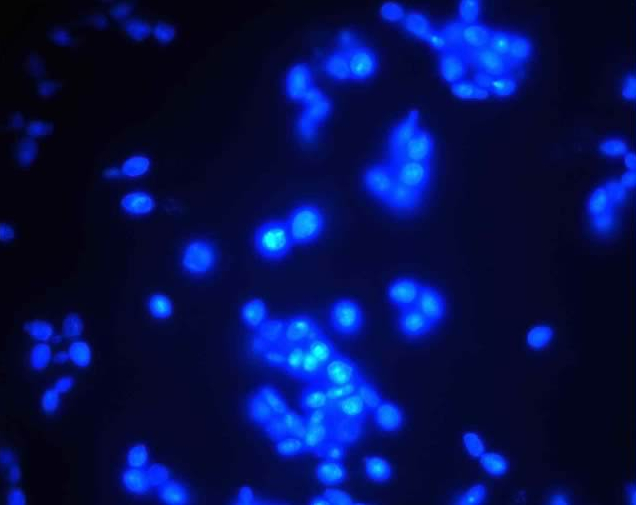
\includegraphics[scale=.55]{img/CAP3bordi.jpg}
 \caption{\small{Immagine in colorazione DAPI di cellule di lievito osservate al microscopio a fluorescenza: ben evidente la disomogeneità spaziale della luminescenza e la presenza di una luminosità residua di sfondo.}}
 \label{fig:bordi}
\end{figure}

Questo programma di correzione della luminosità sfrutta delle sfere nanometrice, di dimensione costante ed intensità di luminosità nota, prodotte appositamente per la calibrazione dei microscopi a fluorescenza.
Esistono diversi set di nanosfere in grado di coprire ampi range di intensità, così da poter creare una curva di calibrazione dall'intensità del segnale osservato (dipendente ad esempio dalla luminosità dell'irraggiamento e dal tempo di esposizione) alla concentrazione di fluoroforo sottostante.
 
Nel nostro caso si è sfruttato il kit di sfere nanometriche fluorescenti nel rosso ``InSpeck Microscope Image Intensity Calibration'', acquistate appositamente per la calibrazione del microscopio in uso.
Esso consiste in una fiala di $5\ ml$ di mezzo di sospensione e 7 fiale di microsfere di polistirene atossico aventi differenti intensità relative: 0\%, 0.3\%, 1\%, 3\%, 10\%, 30\% e 100\%.
Tale richiesta nasce dal fatto che l'algoritmo effettua la correzione dell'immagine a fluorescenza delle cellule sfruttando l'ulteriore acquisizione di due immagini di calibrazione: una di sferette aventi stessa intensità e l'altra di sferette con 5 intensità distinte.

Descriviamo dunque passo a passo le fasi principali dell'algoritmo, riportato nella sua interezza in Appendice A, che possono essere schematizzate in:
\begin{enumerate}
 \item rimozione delle disomogeneità ai bordi dell'immagine,
 \item rimozione della fluorescenza di background,
 \item correzione dell'immagine bersaglio.
\end{enumerate}


\section{Rimozione delle disomogeneità di illuminazione}

Come precedentemente osservato, la disomogeneità di illuminazione comporta immagini a microscopia a fluorescenza con maggior segnale luminoso nella zona centrale rispetto alle regioni periferiche.
L'algoritmo mira alla compensazione di questa disomogeneità stimando punto per punto il valore di segnale atteso a parità di concentrazione di fluoroforo ed usando questa stima per correggere le stime osservate.
Per far questo necessita di una immagine di calibrazione, ossia di un campo contenente solo nanosfere con un'unica intensità (\figurename~\ref{fig:unaint}).
Tramite questa calibrazione l'algoritmo riesce a eliminare in modo sostanziale la dipendenza dell'intensità dalla posizione del pixel. 

\begin{figure}[p]
 \centering
 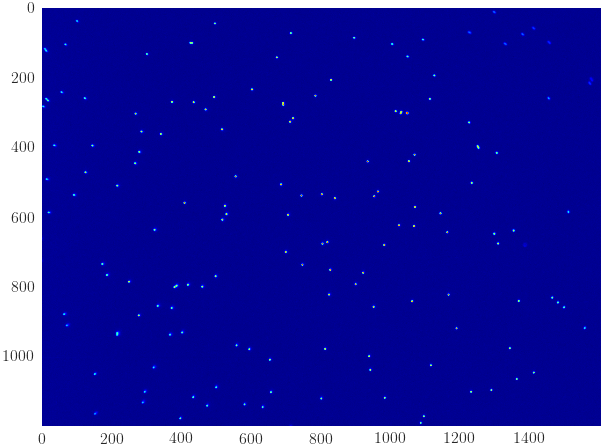
\includegraphics[scale=.64]{img/CAP3unaint.png}
 \caption{\small{Immagine a fluorescenza (1600x1200 pixel) di sferette con intensità relativa del 10\%.}}
 \label{fig:unaint}
\end{figure}

Inizialmente il programma applica sull'immagine il filtro gaussiano, tipico filtro di smoothing molto efficace per attenuare il rumore presente (counting noise dovuto alla bassa intensità delle immagini), e calcola in un primo modo approssimato l'intensità costante residua.
Questo background viene valutato in modo statistico come massimo delle mode, ossia dei valori che compaiono più frequentemente, di ogni riga della matrice bidimensionale che costituisce l'immagine. 
Tale parametro viene quindi sottratto a quest'ultima poiché valore costante in grado di alterare considerazioni quantitative.

Una volta rimossa la componente principale dello sfondo, viene stimato il campo di illuminazione incidente, supposto proporzionale al segnale di ciascuna sferetta (che dovrebbe essere altrimenti omogeneo).
Suddetto campo viene stimato tramite il fit, svolto all'interno del codice dalla routine \textit{analyze}, di una funzione pseudo-gaussiana.
Quest'ultima descrive ragionevolmente bene la luminosità osservata e di conseguenza viene usata come campo di luminosità incidente per la correzione del segnale osservato.


\subsubsection*{Ricerca dei massimi}

Il primo step necessario alla stima della funzione di illuminazione è la ricerca delle nanosfere nell'immagine.
Quest'ultime sono approssimabili come punti di luminosità diffusa, distribuiti in modo gaussiano intorno al punto centrale.
Tali luminosità vengono ipotizzate tutte proporzionali all'intensità luminosa e la possibilità che alcuni di questi punti luce siano in realtà la sovrapposizione di più sfere in contatto viene gestita nel momento del fit.

La ricerca dei massimi viene svolta dalla routine \textit{find\_max}, che prende in input tre parametri: \textit{vicinanza\_size}, \textit{soglia} e \textit{margine}.
Il primo (\textit{vicinanza\_size}) dà la dimensione in pixel dell'area sfruttata dai filtri per la ricerca dei massimi e dei minimi relativi, perciò dovrà assumere valori minori al crescere della concentrazione delle sferette, ma approssimativamente simili al diametro delle nanosfere nell'immagine. 
Il secondo (\textit{soglia}) indica quale debba essere il minimo valore di cui il massimo individuato debba superare il valore del background nei dintorni, per evitare di includere nel conteggio dei massimi dati da effetti di rumore.
Di conseguenza tale parametro dipende dalla luminosità delle sferette: maggiore sarà quest'ultima e maggiore dovrà essere il suo valore.
Dalla ricerca dei massimi viene escluso, successivamente alla determinazione dei punti di massimo (localizzazione ed intensità di ciascuna nanosfera), il confine dell'immagine, utilizzando il parametro \textit{margine}.
Esso indica la larghezza in pixel del bordo da rimuovere dalla stima, così da evitare di includere immagini parziali di nanosfere che potrebbero distorcere il fit.
Difatti ogni sferetta non viene rappresentata come punto oggetto, bensì con un cerchio di confusione (capitolo 2.2.1) e di conseguenza, nel caso in cui l'alone sia a cavallo del margine dell'immagine, potrebbe venire riconosciuto come massimo un punto che in realtà non è il centro della sferetta ma un pixel della sfumatura circostante.

Sempre all'interno di \textit{find\_max} viene associata ad ogni punto di massimo un'intensità integrale media. 
Questa viene calcolata richiamando la funzione \textit{intensity}, la quale somma i valori dei pixel che costituiscono la sferetta e divide il tutto per il numero totale di pixel contati, così da tener conto del fatto che non si tratta di un punto oggetto privo di dimensioni, bensì di un'area con una certa estensione. 
Per fare ciò ovviamente è necessario valutare il raggio \textit{delta} della sferetta, nel nostro caso stimato pari a 5 pixel (\figurename~\ref{fig:punto}).

\begin{figure}
 \centering
 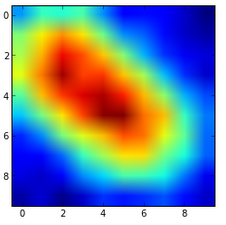
\includegraphics[scale=.25]{img/CAP3punto.png}
 \caption{\small{Selezione di una singola sferetta del kit ``InSpeck Microscope Image Intensity Calibration'' per la valutazione della dimensione associata.}}
 \label{fig:punto}
\end{figure}

\subsubsection*{Fit di maximum likelihood}

A questo punto, avendo identificato i massimi dell'immagine, si stimano i parametri della funzione di illuminazione tramite un metodo di \textit{maximum likelihood}, utilizzando un metodo pre-esistente nel modulo scipy di python, chiamato \textit{curve\_fit}.

Per poter comprendere come venga eseguita questa tipologia di fit, prendiamo un campione casuale $\mathbf{X_n}$ di $n$ osservazioni che può assumere diversi valori, ciascuno dei quali costituisce un campione osservato $\mathbf{x_n}$.
Venga inoltre definito un modello statistico per il campione $\mathbf{X_n}$, ossia una distribuzione $f_n (\mathbf{x_n};\theta)$ con $\theta \in \Theta$ parametro (o insieme di parametri) che identifica la legge di probabilità relativa all'esperimento in corso.
Sulla base di tali identificazioni si definisce funzione di verosimiglianza (likelihood function)
associata ad $\mathbf{x_{oss}}$ la funzione $L_{x_{oss}}: \Theta\longmapsto \Re_+$ tale che:
$$L_{x_{oss}}(\theta)=f_n (\mathbf{x_{oss}};\theta)=\prod_{i=1}^n f_X (x^{oss}_i;\theta) $$
dove $\mathbf{x_{oss}}=(x^{oss}_1, x^{oss}_2, ..., x^{oss}_n)$ è il campione osservato. 
La likelihood function è utilizzata solitamente per condurre tre tradizionali procedure:
\begin{itemize}
 \item ottenere una stima puntuale di $\theta$,
 \item ottenere una stima per intervallo di $\theta$,
 \item scegliere tra due possibili ipotesi riguardanti valori di $\theta$.
\end{itemize}
Il fit di maximum likelihood, utilizzato nell'algoritmo, è volto ad ottenere la stima puntuale, detta anche stima di massima verosimiglianza (MLE). 
Con tale termine si indica il valore $\hat{\theta}$ in cui la funzione di verosimiglianza raggiunge il massimo assoluto, ossia:
$$MLE = \hat{\theta}\ se\ L_{x_{oss}}(\hat{\theta})=\max_{\theta \in \Theta} L_{x_{oss}}(\theta)$$
Detto in altri termini, il punto di massimo della funzione di verosimiglianza è il valore più plausibile di $\theta$ alla luce del campione osservato $x_{oss}$.

Dopo varie analisi si è notato che la funzione che al meglio descrive il comportamento dei massimi di intensità è proporzionale ad una gaussiana multivariata, descritta all'interno della funzione \textit{gauss} tramite la relazione:
$$ G = bg + maxint \cdot \exp \{ {-\frac{1}{2} [{     (\frac{x-cx}{dsx})^2   +  (\frac{y-cy}{dsy})^2  +  \frac{corr \cdot (x-cx) \cdot (y-cy)}{dsx \cdot dsy} ]}^{\frac{e}{2}}}\} $$
dove $bg$ è il parametro di background, $maxint$ è l'intensità massima, $cx$ e $cy$ sono rispettivamente i centri delle coordinate x e y, $dsx$ e $dsy$ sono rispettivamente le deviazioni standard delle coordinate x e y, $corr$ è il parametro di correlazione tra x ed y ed infine $e$ è l'esponente.
Facendo riferimento alla trattazione precedente, $G$ corrisponde alla funzione di verosimiglianza $L_{x_{oss}}(\theta)$, ove $\theta$ in tal caso è l'insieme dei parametri $(bg,\ maxint,\ cx,\ cy,\ dsx,\ dsy,\ corr,\ e)$.
Essendo questo uno dei punti cardine della correzione, si è deciso di parallelizzare la funzione \textit{gauss}, così da avere un guadagno nei tempi dell'ordine di quattro volte.

\begin{figure}
 \centering
 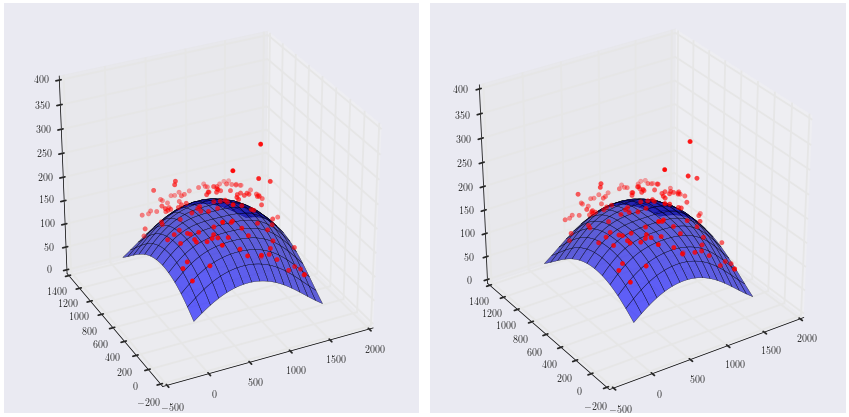
\includegraphics[scale=0.45]{img/CAP3gauss.png}
 \caption{\small{Immagine in visione ``cross eyed stereoscopic'': i puntini rappresentano i massimi della \figurename~\ref{fig:unaint} mentre la superficie è quella risultante dal fit di maximum likelihood.}}
 \label{fig:gauss}
\end{figure}

\begin{figure}[p]
 \centering
 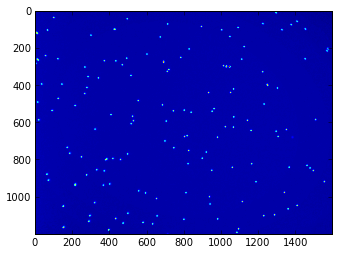
\includegraphics[scale=.64]{img/CAP3unaintcorr.png}
 \caption{\small{Immagine risultante dalla correzione della disomogeneità di campo sull'immagine in \figurename~\ref{fig:unaint}.}}
 \label{fig:unaintcorr}
\end{figure}

Una volta ottenuta la stima di massima verosimiglianza, ossia il set di parametri in grado di massimizzare la likelihood function, ciò che si viene a creare è una superficie tridimensionale con forma analoga a quella riportata in \figurename~\ref{fig:gauss}. 
Quest'ultima immagine mette bene in evidenza il fatto che alcuni punti di massimo corrispondono ad intensità molto elevate rispetto alla media, pur trattandosi di sferette con medesima intensità relativa.
Questo fenomeno è da associarsi alla possibilità che due sferette possano trovarsi così vicine da apparire sovrapposte e, essendo questa un'alterazione dei risultati, è necessario rieseguire il calcolo dei parametri dopo aver eliminato tali punti più intensi. 
Per fare ciò viene utilizzato il quantile$_{0.95}$ dei massimi normalizzati, ossia vengono eliminati dal nuovo fit quei pixel con intensità superiore ad esso, pari per definizione al 5\% dei massimi inizialmente rilevati.
I nuovi parametri ottenuti a questa seconda iterazione sono restituiti dalla funzione \textit{analyze} e sono utilizzabili per la correzione delle disomogeneità nelle regioni periferiche dell'immagine di una qualunque immagine a fluorescenza rilevata con lo stesso apparato, inclusa la stessa di calibrazione (\figurename~\ref{fig:unaintcorr}).
Infatti a questo punto, inserendo una qualsiasi immagine come variabile di ingresso della funzione \textit{correction}, è possibile eliminare tale difetto sfruttando unicamente la stima di massima verosimiglianza precedentemente calcolata. 
Tale funzione è molto semplice poiché sfrutta la normalizzazione del valore dei pixel dell'immagine sulla base del valore previsto dalla superficie tridimensionale, rinormalizzando il segnale osservato per la funzione di intensità di illuminazione ottenuta.



\section{Rimozione della fluorescenza di background}

La seconda immagine di calibrazione, costituita da nanosfere aventi differenti intensità (\figurename~\ref{fig:piuint}), viene sfruttata per correggere il problema della fluorescenza residua di sfondo, tramite il controllo della risposta lineare dello strumento. 

\begin{figure}[p]
 \centering
 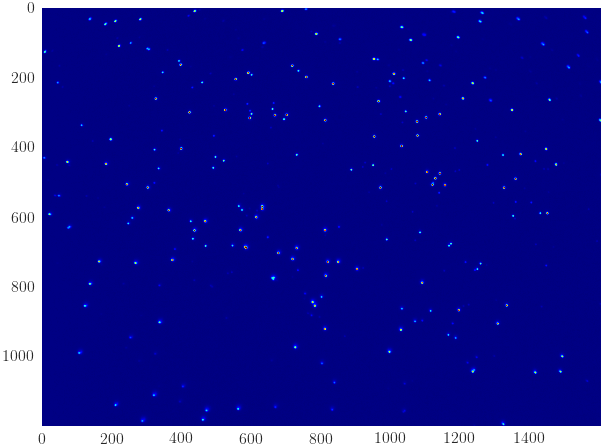
\includegraphics[scale=.64]{img/CAP3piuint.png}
 \caption{\small{Immagine a fluorescenza (1600x1200 pixel) di sferette con cinque differenti intensità relative: 1\%, 3\%, 10\%, 30\% e 100\%.}}
 \label{fig:piuint}
\end{figure}

Come nella prima fase dell'algoritmo, all'utente viene richiesto di inserire la seconda immagine di calibrazione.
A questa viene applicato uno smoothing gaussiano e sottratto il parametro del background. 
Successivamente, sulla base dei parametri del fit calcolati tramite la prima immagine di calibrazione viene corretta la disomogeneità di illuminazione.

A questo punto ai fini del controllo della risposta lineare del microscopio, vengono riconosciute nell'immagine le curve gaussiane relative alle differenti intensità. 
Nel nostro caso sono stati inseriti nel campione cinque diversi tipi di sferette, escludendo quelle con intensità relativa del 0.3\% poiché non sufficientemente intensa intensa, e di conseguenza vengono riconosciute cinque distinte curve gaussiane.
Queste sono state identificate tramite un \textit{Gaussian Mixture Model (GMM)} sul logaritmo delle intensità, nel quale le intensità sono distribuite in modo approssimativamente regolare con deviazione standard e numero di osservazioni simili fra le varie gaussiane. 
Di ciascuna di questa viene registrata la media, la deviazione standard e la numerosità.
Il fit è stato effettuato tramite la funzione per le \textit{Gaussian Mixture Model (GMM)} presente nella libreria \textit{scikits-learn}.
Un esempio dell'istogramma delle intensità risultante e del relativo fit si può vedere in \figurename~\ref{fig:istogauss}.

\begin{figure}
 \centering
 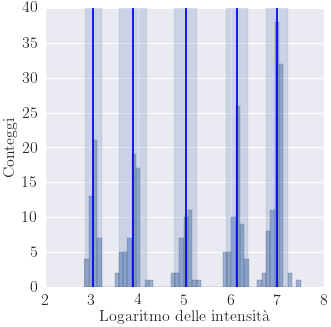
\includegraphics[scale=.60]{img/CAP3istogauss.png}
 \caption{\small{Istogramma delle cinque curve gaussiane corrispondenti alle intensità dei massimi presenti nella seconda immagine di calibrazione, una volta corretta dalla disomogeneità di illuminazione. La linea marcata e l'area sfumata presenti su ogni curva rappresentano rispettivamente il valore medio e la deviazione standard della gaussiana, identificati dalla GMM.}}
 \label{fig:istogauss}
\end{figure}

I valori medi delle gaussiane rappresentano le intensità medie di ciascuna categoria di sferette e di conseguenza, essendo queste comunque note a priori, è possibile creare una regressione lineare tra le intensità previste e quelle effettivamente rilevate all'interno del campione, così da controllare la linearità della risposta e correggere di conseguenza il parametro di background. 
Un primo fit lineare è stato fatto sfruttando la funzione \textit{linregress}, la quale restituisce un array contenente in particolare la slope e l'intercetta della curva di fit e la correlazione esistente tra i due set di dati in esame.
Come si evince dalla \figurename~\ref{fig:linearita}, la relazione tra intensità rilevate e note sembra non essere perfettamente lineare. Infatti il grafico in scala logaritmica presenta una slope non identicamente unitaria, pari a 0.87, e quello in scala lineare mostra una leggera curvatura dell'andamento dei dati. 
Inoltre le incertezze associate ai dati in esame, sebbene riportate nel grafico, risultano impercettibili, ulteriore indice del fatto che questa  difformità dalla linearità non è frutto del caso.
Ad ogni modo la discrepanza risulta essere non troppo evidente e trattabile con una trasformazione non lineare semplice dell'intensità dell'immagine; per tale motivo, in prima approssimazione, possiamo ignorare eventuali non-linearità e considerare perciò verificata l'ipotesi di risposta lineare del microscopio. 

\begin{figure}
 \centering
 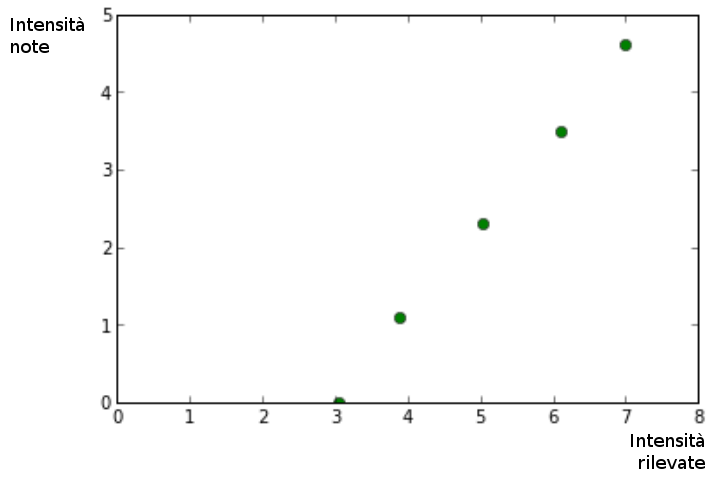
\includegraphics[scale=.55]{img/CAP3linearita.png}
 \caption{\small{Grafico con incertezze (non percettibili) delle intensità medie delle cinque gaussiane corrispondenti ai massimi della seconda immagine di calibrazione corretta dalla disomogeneità di illuminazione in funzione di quelle note ed associate rette di regressione lineare. Sulla sinistra è riportato il grafico in scala logaritmica, mentre sulla destra in scala lineare.}}
 \label{fig:linearita}
\end{figure}


\begin{figure}[p]
 \centering
 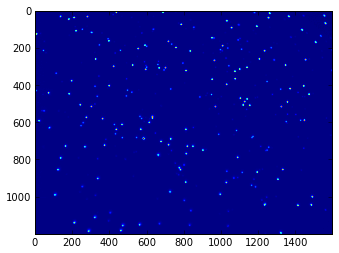
\includegraphics[scale=.64]{img/CAP3piuintcorr.png}
 \caption{\small{Immagine risultante dalla correzione della disomogeneità di illuminazione e della fluorescenza di background sull'immagine in \figurename~\ref{fig:piuint}.}}
 \label{fig:piuintcorr}
\end{figure}

Sulla base di tale ipotesi l'unico obiettivo rimasto risulta essere la rimozione del valore costante della fluorescenza di sfondo. 
Per fare ciò basta occorre traslare i valori in modo da ottenere il passaggio della retta di regressione dall'origine, ossia a livello pratico è necessario sottrarre all'immagine l'intercetta calcolata. 
Essendo questo un altro pasaggio cardine dell'algoritmo, si è scelto di rivalutare l'intercetta all'origine in modo più preciso, ossia tramite un secondo fit lineare eseguito con un'apposita funzione di \textit{curve\_fit}.
A questo punto per la rimozione della fluorescenza di background basterà semplicemente sottrarre il parametro dell'ordinata all'origine all'intera immagine presa in considerazione. 
L'immagine di calibrazione usata per correggere questo secondo difetto può essere a sua volta autocorretta, come mostrato in \figurename~\ref{fig:piuintcorr}.

Tramite questa seconda fase, che sfrutta l'immagine di calibrazione di nanosfere con differenti intensità e i parametri del fit di maximum likelihood ottenuti nella prima fase, si riesce quindi a eliminare in modo sostanziale l'ulteriore difetto della fluorescenza residua. 


\section{Correzione dell'immagine}

La parte finale del programma è volta alla correzione di entrambi i difetti, l'illuminazione disomogenea e la fluorescenza residua, per una qualsiasi immagine acquisita con il microscopio a fluorescenza (\figurename~\ref{fig:cell}). 

\begin{figure}[p]
 \centering
 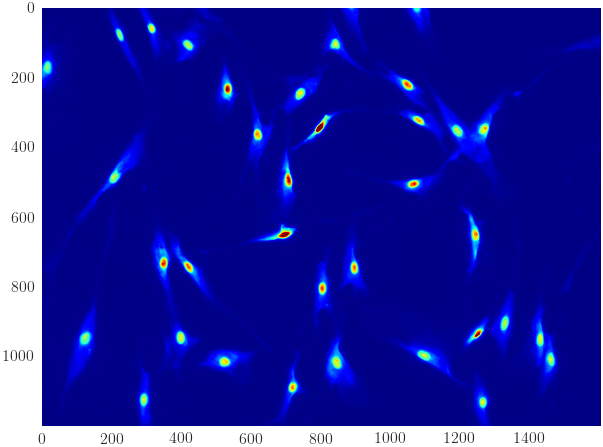
\includegraphics[scale=.64]{img/CAP3cell.png}
 \caption{\small{Immagine a fluorescenza di fibroblasti primari. Si può notare come i nuclei presenti al centro dell'immagine risultino più intensi (maggior componente rossa) rispetto a quelli vicini alla periferia.}}
 \label{fig:cell}
\end{figure}

A questo punto l'algoritmo richiede da parte dell'utente l'inserimento di una terza ed ultima immagine a fluorescenza, quella su cui si vuole fare un'analisi quantitativa e quindi che necessita della correzione.
Ad essa, come per le precedenti, viene inizialmente applicato il filtro gaussiano e sottratto il valore approssimato di background.

La prima correzione ad essere effettuata sull'immagine è la rimozione della fluorescenza residua di sfondo. 
Difatti le viene sottratto il valore dell'ordinata all'origine calcolato tramite la seconda immagine di calibrazione, contenente il mixture di sferette.

Successivamente viene rimosso il difetto dei bordi sfruttando la funzione \textit{correction}, ossia vengono messi in gioco i parametri calcolati dal fit di maximum likelihood tramite le sferette ad una sola intensità.

Giunti a questo punto l'immagine si può ritenere corretta (\figurename~\ref{fig:cellcorr}) e di conseguenza risulta sicuramente più precisa una qualsiasi misura quantitativa eseguita su di essa.

\begin{figure}[p]
 \centering
 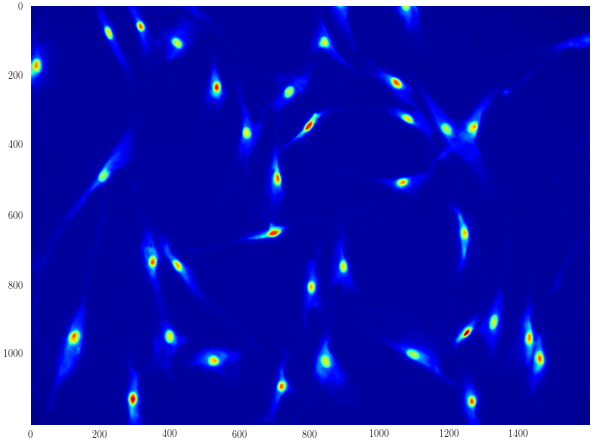
\includegraphics[scale=.64]{img/CAP3cellcorr.png}
 \caption{\small{Immagine risultante dalla correzione della disomogeneità e della fluorescenza di background sull'immagine in \figurename~\ref{fig:cell}. Si può notare (qualitativamente) come i nuclei periferici abbiano assunto un valore più simile a quelli centrali, con un maggior contrasto rispetto allo sfondo.}}
 \label{fig:cellcorr}
\end{figure}